\documentclass{style/CRPITStyle}
\usepackage{epsfig}   % Packages to use if you wish
\usepackage{lscape}   %
\usepackage[authoryear]{natbib}
\renewcommand{\cite}{\citep}
\pagestyle{empty}
\thispagestyle{empty}
\hyphenation{roddick}

\begin{document}

\title{Software Development Life Cycles: History and Future}
\author{David Barnett}
\affiliation{School of Engineering and Computer Science \\
Victoria University of Wellington, \\
PO Box 600, Wellington, 6140 \\
Email:~{\tt barentdavi@myvuw.ac.nz}}

\maketitle

\begin{abstract}
    % TODO
    Abstract goes here
\end{abstract}

\vspace{.1in}

\noindent {\em Keywords:} Software Process Models

\vspace{.1in}

% \section{Introduction}
% TODO
% thesis statement

\section{Importance of using process models}
% Q: describe the importance of using process models to guide software development

% why we need process modeling
Fail to plan, is a plan to fail. 
As software has increased in complexity and scale of projects increase it
became more apparent that software should be managed and planned differently it was
described as a \emph{Software crisis} \cite{nato:1969}.
``We believe that the only way ahead lies through the steady development of the best existing 
techniques'' \cite{nato:1969} Gill's comments on how to move forward from the
\emph{Software Crisis} which describes a need for more of an engineering approach to software development.
One such endeavour is process modelling.
A process model is a model of how to setup a project with a set of tasks,
such as requirements acquisition or construction, of a similar nature that together form 
the scaffolding of a plan of how to approach to build a project.

\paragraph{} % are we allowed to do this?

By using the appropriate process model software development can be guided
through the many stages of creating software with an over-arching idea of how it
should be done. This can range from having static requirements and working
linearly through the development cycle to changing the requirements from week to
week. With the right processing model the software will have the correct tools
to handle what was expected to happen through out the process and give a guide
through the unexpected.

% add more on why it is important and how it guides

\section{Review of Process Models}

% TODO: this needs some reworking
Over the years many process models have been proposed and many variations have
been used and reported one. The process models that will be discussed in this
review is: Waterfall, V-Model, Spiral Model, Iterative and Incremental Development and
Extreme programming.

% --- 5 Model Section ---
% Q: provide a systematic review of process models that have been proposed so far,
% Q: compare and contract 5 selected distinct process models for software development
% Q: identify central themes that have been considered important for evolving process models
\subsection{Waterfall} % sequential
% theme: sequential
% strengths: requirements up front, easy
% Goals: a model of how to make successful large software
% Strengths: easy, clear steps and deliverables
% compare: ??
% contrast: ??
% note: Need a counter source, "Enough with Life cycle?"

% should include an overview & theme of the model
The Waterfall model was proposed in 1970 by Dr. Winston Royce \cite{royce:1970:waterfall} 
with a focus on meeting requirements.
He proposed it as a method to be a guide of steps and processes that together
help to make a larger software project succeed. 
The principle idea behind the Waterfall model is that there are seven stages to
software development cycle and they are to be executed in a sequential order:

\begin{enumerate}
  \item System requirements
  \item Software requirements
  \item Analysis
  \item Design
  \item Coding
  \item Testing 
  \item Operations
\end{enumerate}

The end of each stage is a milestone of how the project is progressing and with some artifacts
that the next stage depends on, making them static for simplicity, and builds upon
them to deliver the next milestone till the product at the end of the process is
complete.

\vspace{.1in}

\begin{figure}[htb]
\fbox{\parbox[b]{.99\linewidth}{
\vskip 0.5cm
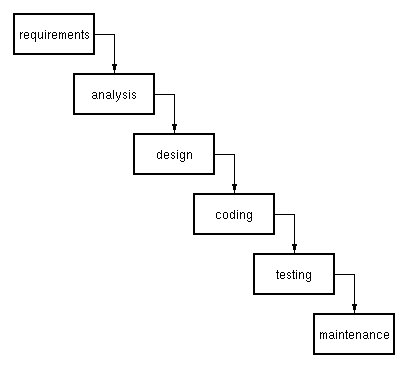
\includegraphics[width=0.45\textwidth]{figures/waterfall-model.png}
\vskip 0.5cm}}
\caption{\protect\label{waterfall}  Waterfall Model}
\end{figure}

\vspace{.1in}

Figure 1 shows the general form that Waterfall takes with its characteristic 
linearly moving between each stage with no movement back to previous stages of
development.

\paragraph{}

% main features of waterfall
The strength of this model lies in the assumptions that the requirements are
well thought out, any foreseeable problems has known solutions to complete the
software.
This lends the model to be more suitable for software projects that have well known
requirements and technology such as porting an application to another platform.
Waterfall also has the benefits of being an easy project to manage with its
clear milestones of development and equally easy for a new member or external
stakeholder to the team to understand the status of the project.
This allows the size of the project team to scale up very large and still be
effective in managing.

\paragraph{}

% covers the weakness of water fall
Conversely the strengths of the model also highlights the weaknesses of the model as
well.
One of the assumptions in the process model is that the requirements at the start of the project is
static and are still meet the clients needs that the project was started for.
Another factor to this weakness is that the model allows for only one delivery of the product to
the client at the end of the whole project, making a possible large time gap from requirements 
gathering with the client to the final delivery to the client which has the risk of not being 
what the client had in mind during the initial phases of the project
\cite{McCracken:1982}.

\paragraph{}
Though in spite of the downside of Waterfall, it has some valid use cases.
The main use case is when the requirements for the project is well known and the
solutions to the problems are also known and solved and that risk is not a large
enough factor that a model better suited to handle it, such as V-Model or Spiral
Model should be chosen, then Waterfall is a good choice for a process model.
Waterfall could also be used in large teams as it is a simple process to follow
and can scale to a large team size.
Examples of a good projects to Waterfall are porting applications or government
work.

\subsection{V-Model} % sequential, testing
% theme:
% Goals: to extends the existing Waterfall to include testing
% compare: Waterfall's steps
% contrast: Has testing involved in the 

% should include an overview & theme of the model
V-Model was proposed as a variation of the Waterfall model by Paul Rook in 1986
\cite{rook:1986:vmodel} with a testing focus.
The principle idea of the V-Model is to produce software in a linear fashion with
well known requirements and solved problems that has the need for extensive testing 
and verification of the system \cite{rook:1986:vmodel}.
The general workings of the V-Model are similar to the workings of Waterfall
with a few differences in testing.
Instead in V-Model the testing stage of the process model is expanded and added short loops,
the software is tested against the produced designs and requirements with
steps of verification and validations  that if failed will lead back to the design
stages or requirements respectfully.

\vspace{.1in}

\begin{figure}[htb]
\fbox{\parbox[b]{.99\linewidth}{
\vskip 0.5cm
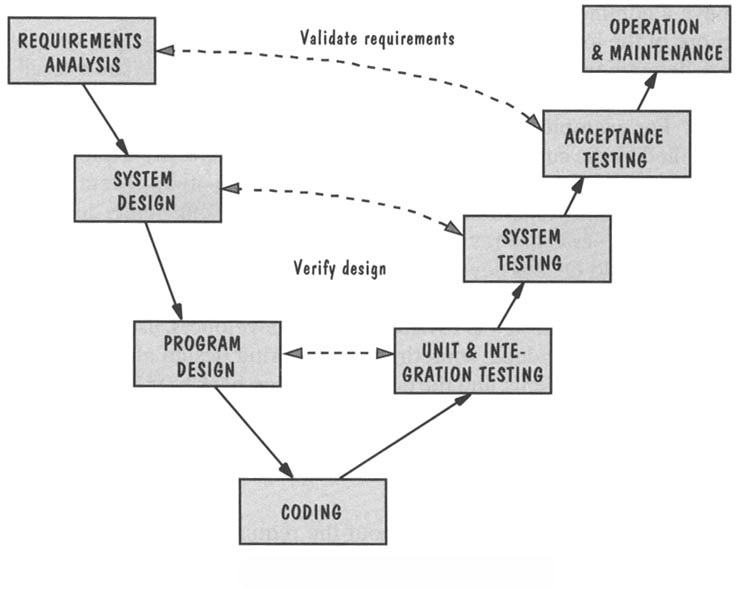
\includegraphics[width=0.45\textwidth]{figures/v-model.jpg}
\vskip 0.5cm}}
\caption{\protect\label{vmodel}  V-Model}
\end{figure}

\vspace{.1in}

Figure 2 shows a common interpretation of V-Model with its characteristic
building of requirements and designs to be tested against on the left side of
the model leading to the building of the software then moving up the right side
verifying and validating the software built against the specification built
earlier. Failure to meet leads back to the appropriate to re-visit building that
level of the design or the specification. Finally at the end releasing the
product to the client.

\paragraph{}

The strengths of the V-Model are built up upon Waterfall.
As with Waterfall, V-Model also is an easy to mange project with clear milestones
to each stage of development.
V-Model splits off from Waterfall with its focus
on verification and validation of the product.
Each artifact from the milestones are also used in the process again with either
being an artifact to test or to test against to verify and validate the product
moving forward. Failing to pass the test will lead back to the stage allowing to
fix a past mistake, recognising that it is hard to get it prefect the first time
round.
Through the testing the V-Model has the potential to produce an extensively well
tested product that meets a set of strict requirements such as traffic networks
or medical equipment \cite{advancements:2010:vmodel}.

\paragraph{}

% needs a cite in it somewhere
The shortcomings of V-Model as well is akin to Waterfalls.
V-Model relies upon the requirements are quite static but has slightly more
flexibility than Waterfall due to the addition of more extensive testing that introduced loops 
through the verification and validation processes of the product. 
The extensive testing is only truly beneficial given that the project needs to
be tested to such lengths, in situations that the end-product is used in safety
critical situations the testing will be a great asset but for other types of
projects that do not need a high level of verification and validation it would
be an expensive use of resources on an area for little benefits.
However this does not allow V-Model to be as flexible as iterative process models such as
Agile based models as V-Model still have a large time period between project
initiation and delivery. 
V-Model also suffers from the same fate of Waterfall in the fact that it only
delivers a single version of the product to the client. Which carries a risk of 
not meeting the clients needs, though it is indirectly managed through the validation testing.
This is an inherent risk of only delivering a single version at the end
of project common in sequential process models like V-Model and Waterfall.
V-Model also suffers the same problem as Waterfall in the fact it does not 
have as much client involvement as iterative models such as Incremental and
Iterative development model.

\paragraph{}
The V-Model's use cases are a subset of Waterfall as it targets a sub-set that
requires an extensive amount of testing.
The V-Model is only appropriate when all the requirements are known upfront and
the solutions to the problems the requirements presents are known and solved.
This makes V-Model have a strong use
case in safety critical system that require reliability, safety and security.


\subsection{Spiral Model} % sequential / Iterative, testing, risk
% theme: sequential / iterative, risk
% compare:
% contrast:

The Spiral Model is a process model that Barry Boehm described in 1986 \cite{boehm:1988:spiral}.
The model has a mixture of ideas in it, the core idea of the model is to address risk management and analysis
which neither Waterfall or V-Model directly tackled.
Spiral model also shares some ideas from both Waterfall and V-Model with a sequential approach 
but also includes some iterative elements with producing multiple prototypes of the 
product over the course of the whole project but only delivers a single product
at the end of the development.
The rest of the process progresses linearly going through the software 
development cycle with the addition of steps to review and plan for
the next iteration of the prototype as well as identifying risks and
how to resolve them going forward.

\vspace{.1in}
\begin{figure}[htb]
\fbox{\parbox[b]{.99\linewidth}{
\vskip 0.5cm
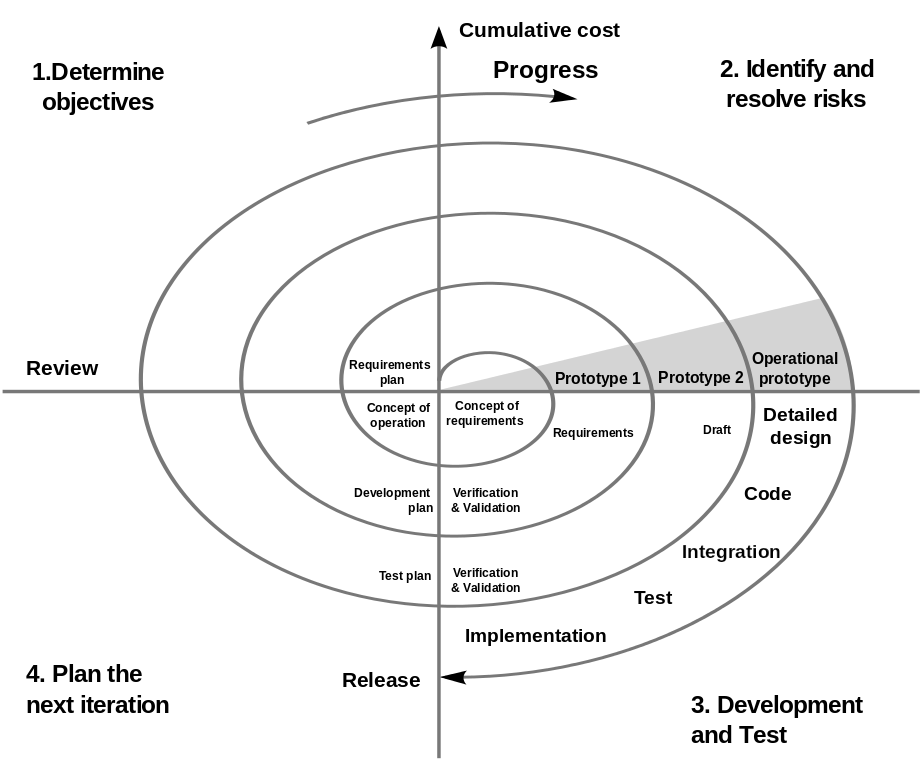
\includegraphics[width=0.45\textwidth]{figures/spiral-model.png}
\vskip 0.5cm}}
\caption{\protect\label{spiral}  Spiral Model}
\end{figure}

\vspace{.1in}

Figure 3 shows the general use of the Spiral Model, with some simplifications, 
with multiple cycles or iterations \cite{boehm:1988:spiral}.
Each cycle of the spiral starts with the identification of highest risk parts of the
final product to be developed in this iteration, shown as quadrant one in figure 3. 
This process also includes suggesting alternative ways to implement what
has been identified and
identifying the resource constraints for the cycle.
The next quadrant's goal is to handle risk analysis and resolving the identified
risk, allowing ``risk-driven subsetting of the spiral model steps allows the model 
to accommodate any appropriate mixture of a specification-oriented, 
prototype-oriented, simulation-oriented, automatic transformation-oriented, 
or other approach to software development'' \cite{boehm:1988:spiral}.
Which lends Spiral model to be very flexible with its application.
The third quadrant is the execution of the planning for the cycle with
development, testing and verification of the produced prototype form the
iteration. 
The final quadrant is to review the work that has been done including key
stakeholders in the review process.
% finish the overview of Spiral ^
% Done: 1, 2, 3, 4 

\paragraph{}

% Explicitly state Strengths + themes, cite!
The strength of the Spiral model comes from its ability to be
flexibility with how the project can be focused on a range of
different aspects such as specification or prototype.
Another strength is its ability to monitor and control through the whole process
of the development, which allows the project to explore solutions to problems
where in Waterfall or V-Model will be force to stick to the tried and true
methods instead of having the potential to innovate as spiral does.
With the inclusion of iterations Spiral has a large benefit of getting user and
client feedback during the development process to ensure the final product meets
the client's on important aspects such as user interface. This is a large
advantage above sequential models such as Waterfall that do not include any
explicit user interface iteration and refinement.

\paragraph{}

% cites plz
With the benefits and flexibility that the Spiral Model offers it comes at a
cost. 
One of them are the complexity to manage a project with Spiral, the process of
repeated iterations involve a considerable amount of overhead and repeated work
that is saved in Waterfall or V-Model. One such
problem is falling into the trap of running each cycle of the spiral as if it
was a miniature Waterfall.
The iteration are excellent for tracking the progress of the project but not all
projects benefits can be completed in parts and must be completed holistically
such as software supporting critical infrastructure where a sequential model
like V-Model is better suited.
Another cost of Spiral model is the need to have an expert of the risks that
will be needed to be identified and resolved which could cause a large strain on the
resources of the project than the benefits of mitigating the risks.

\paragraph{}
With the costs and benefits of the Spiral model it has many different use cases.
The most prominent use case of the Spiral model is when risk analysis,
evaluation and management is an important component of the development of the
software. It also has a use case of when a prototype of the final software
product is useful, such as when a user interface for the software is needed.
Spiral model is appropriate to be used with research or extermination with a new
product as it allows for multiple prototypes with a single focused goal 
to deliver at the end with a tools in place to handle the changes and 
risks involved with pushing new developments in areas.
Spiral model also handles a complex set of requirements as it allows chances to
realign the project with the clients expectations with the prototyping.

\subsection{Iterative and Incremental Development} % iterative, testing, risk
% theme: iterative, many deliverables, evolutionary
% goal: to build a working product every cycle and build upon it
% compare: Spiral
% contrast: Waterfall

Iterative and incremental development (IID) model is unsurprisingly an iterative take on the
process model that has the main goals to deliver a small sections of the program
over the course of the development rather than a monolithic delivery which is
common in sequential process models such as Waterfall \cite{greer:2004:iid}.
Iterative development has an idea used in other industries such as aerospace to 
great effect and was thought to be applied to software in 1982 \cite{larman:2003:iid}.
The IID model is a combination of an iterative method with an incremental build
model that seeks to deliver the highest priorities to the client first and then
precede to increment upon implementing the next most important feature.

\vspace{.1in}

\begin{figure}[htb]
\fbox{\parbox[b]{.99\linewidth}{
\vskip 0.5cm
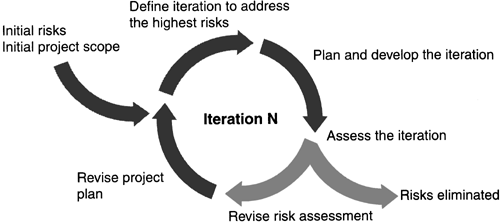
\includegraphics[width=0.45\textwidth]{figures/iid-model.png}
\vskip 0.5cm}}
\caption{\protect\label{iid} Iterative and incremental development Model}
\end{figure}

\vspace{.1in}

% talk to the figure!

\paragraph{}

%% Strengths
% CITE!
The strength of the Iterative and incremental development model is shown when it
is used in a project that benefits from delivering small portions to the client
as the development process unfolds. With the IID model developing the highest
priority first it ensures that each iteration on the software product delivers
more value to the client, allowing to the client to use the partially complete
that have the necessary functionality needed for the client.
This shows how the IID model is more client focused with the need for
prioritized lists of functionality which has the advantage to be flexible to
adapt to an ever changing set of requirements for the client.

\paragraph{}

The flexibility leads to lower committal of upfront resource as the development
can stop at the end of any iteration which allows for a software project to be
developed till it no longer becomes a viable product.
This allows the client to reach a newly developing market faster, where other
models such as V-Model or Waterfall will have a large time-gap and may even miss
the client's goals as the market may of changed since the requirements
collections at the start of the project.

\paragraph{}

With the clients having input on each iteration with the prioritization of
features for the next round of iteration it allows them to have a more hands on
approach to the direction of the product as a whole and they can respond to
changes they want to see in the product as it grows with each iteration.

\paragraph{}

With all the flexibility between iterations during one the requirements are
static, as if it is a miniature waterfall to produce the next increment of the
system, this helps to manage the risk of requirements changes mid-development
by moving the only time it is acceptable to the planning phase with the client.
As with each iteration the focus of the iteration could change to focus on one
type of features, such as performance, that would require only a single area
of expertise so the project could be structured to have rolling experts on the
project for only the times where they are needed or phase out and in development
teams to complete specialised sub-systems in the product.

\paragraph{}

%% Weakness
% cite!
There are some shortcomings of using the iterative and incremental development model.
While having so much interaction and involvement with the client is the time
commitments the client needs to give to the project.
With only delivering the highest ranked priorities each iteration the client or end users may not be
satisfied with using an incomplete product that could have large changes every
iteration which could make it a moving target for end user training on the
product \cite{sommerville:1996}. This is a concern in iterative development where in sequential model
like Waterfall would deliver a complete solution to the client and the end-users
without the risk of having to relearn or adapt to changes in the product over
the whole development period.

\paragraph{}
Under iterative and incremental development model the could project never with
an ever expanding scope that requires more and more feature that the client
desires, in similar process models such as Spiral model or in sequential models
such as Waterfall or V-Model this is handled by the entire models developing
towards a fixed project goal.

\paragraph{}
By having to extend and increment the product over many iteration would require
well defined interfaces between modules.
The code base of the software product would need to be well designed to 
allow for the large amount of extensions and iterations on sub systems without
falling into ta trap of code-and-fix which was prevalent in the software crisis
\cite{nato:1969}. This is an issue with not being able to predict the entire
project in the initial architectural design of the product \cite{sommerville:1996}, where when a monolithic
product delivery is used instead of an incremental such as Waterfall, V-Model and Spiral models 
have more upfront architectural designs to manage the risk of having
architectural problems in the extension of the product.

\paragraph{}
Given the strengths and weakness of the Incremental and iterative development
there are some appropriate use cases for the model. A strong use case for IID is
getting a product to market quick to cash in on a new found niche or to get out
before competition. Another use case for the model is when the majority of the
requirements are known at the start of the project with an expectation of some
of them are going to change over time, this will given enough knowledge 
that an effective initial architectural design of whole project can be made and
iterated on over the course of the project while still adapting to the changes
around the product and the client's needs. A long term software project such as
a compiler or a kernel would benefit from an IID approach as the goal of the
project is clear with variations in small details and improvements with new
technology or research can be incorporated as the project moves forward.

\subsection{Extreme Programming} % iterative, testing, risk
% theme: iterative, evolutionary
% compare:
% contrast:

Extreme programming is an \emph{Agile} methodology which tries to avoid
Waterfall's main downfall, monolithic deliveries with an iterative development
and delivery \cite{khramtchenko:2004:xp}.
The extreme programming methodology was introduced by Kent Beck
\cite{beck:2000:xp} with his book \emph{Extreme programming explained: embrace change}.
The objective of Extreme programming is to deliver high quality software and customer satisfaction using
client involvement and an iterative process. The main diver for Extreme programming 
to achieve this objective is through the values that the methodology has:
Simplicity, make the simplest solution that works for now not to solve all possible
future cases ; Communication, including both inside the team and to the clients ; 
and Testing, the requirement is not complete until the appropriate testing is complete \cite{khramtchenko:2004:xp}.

\begin{figure}[htb]
\fbox{\parbox[b]{.99\linewidth}{
\vskip 0.5cm
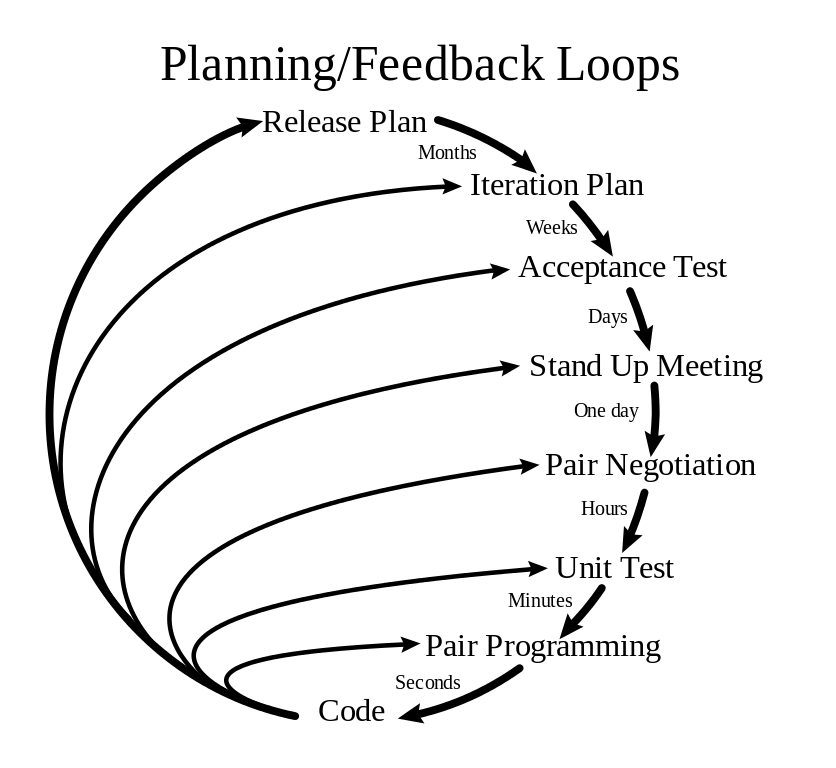
\includegraphics[width=0.45\textwidth]{figures/xp-model.png}
\vskip 0.5cm}}
\caption{\protect\label{iid} Extreme Programming Model}
\end{figure}

% talk to the figure!

\paragraph{}

Figure 5 shows Extreme programming as in the form of a process model.
It shows how Extreme programming breaks down each step of the process down to
coding. This reflects how Extreme programming treats the coding aspect of
the software development cycle to be the very important which is again reflected 
in the processes used to ensure quality, such as ensuring testing by making the
developers who wrote the functionality to write extensive tests for it and
taking code review to the extreme by having a constant code review by pair
programming a feature and subsequent tests \cite{beck:2000:xp}.
The figure shows the 8 key points in Extreme programming, the Release Plan,
Iteration Plan, Acceptance tests, Daily stand up meetings, Pair negotiation,
Unit testing, Pair programming and coding.  
The Release plan is the agreed goal for the next release of the software 
product and what should be delivered over multiple iterations using User 
stories to obtain the requirements from the client in nontechnical language, the
plan may cover multiple iterations over a few months.
The iteration plan is a collection of User stories collected from the release
plan that will be completed over the duration of the iteration cycle which could
cover a small number of weeks.
Acceptance tests are translations of user stories into a technical specification
of which the product can be tested against during the iteration as well in
future iterations to prevent regressions in the product.
Stand up meetings are a short daily meeting held with on-site workers on the project
discussing what they have done, what there are going to do next and what is in
their way. This regular communication to all members, including the client if 
they are on-site, of the current status of the project and how on track it is to
meet the iteration's goals. Peer programming is used as a constant peer review
to ensure quality of the code written, though the pairs swap and change over the
course of days or day.

% strength
\paragraph{}
Extreme programming has many strong points in its model by taking parts of the
development cycle and general project management to the extreme, such ``If code
review are good, we'll code review all the time'' \cite{beck:2000:xp}. As a
result of the peer programming the quality of code produced would make up the
loss of having two programmers at the same computer instead of working on two
different things as the process of peer programming would decrease the
likely hood of bugs, bad architectural decisions and general \emph{code smells}
by continuously discussing the code with the partner as well as aiming to
develop the simplest solution for the current problem like in Incremental and
Iterative development. This is a unique feature
to Extreme programming over the other iterative models such as Spiral or
Incremental and Iterative development model.
Another strength is the entire process is driven by the in-depth communication with
the client and has large client involvement such that the client can writes simple specifications
in the form of user stories and prioritizes which stories make it th the next
release or iteration of the product. This is similar to the Incremental and Iterative
development model as both have heavy client involvement, and to a lesser degree
to Spiral model as the client is not involved to the same extent.
A common trait for a iterative models, one that Extreme programming also has, is
the ability to adapt and be flexible to changes in the clients needs and manages
to deliver on the changes, where V-Model or Waterfall may have great trouble to have
large change of directions.
Another common strength with Incremental and Iterative development is the speed
of which the software is developed, but Extreme programming focuses more on the
quality of the code with the empathise on communication within the project thus
reducing the risk of architectural growing pains that Incremental and Iterative
development may fall into. 
This is also a step to handle the risk that such rapid development faces,
another step is having a strict unit testing of the code and the acceptance tests 
of functionality against user stories in the current and previous
iterations to mitigate the risk of undoing the functionality built in former
iterations.

% weakness
\paragraph{}
All process models have flaws, with Extreme programming one of the come in the
form of management. The progress of the project as a whole is less clear as in
sequential models like Waterfall and can become a difficult project to manage
as the process lacks clear milestones which for a large system could lead to
mismanagement \cite{khramtchenko:2004:xp}. Though the process has measures in
place to mitigate the degradation of code base, mainly peer programming, it 
still faces the same problem as in Incremental and Iterative development with
the risk of large amounts of time wasted due to poor decisions made early in the
development of the product. The model's main empathise on communication does not
scale to larger projects as it becomes increasingly difficult to effectively
use the key communication of stand up meeting with a large number of people,
this is in contrast with models that are simpler to manage such as 
Waterfall \cite{khramtchenko:2004:xp}.

% use cases
\paragraph{}

\section{Possible evolutions of process models}
% Q: try to forecast how current process models may evolve in the future


\bibliographystyle{agsm}
\bibliography{essay}

\end{document}

% vim:set spell et sw=4 ts=4 tw=80:
